\chapter{Definição de escopo da aplicação}

\section{Objetivos do Projeto}
O \textit{FinTrackr} é um aplicativo web responsivo de gestão de despesas pessoais, desenvolvido para proporcionar aos usuários uma ferramenta eficiente para o controle e análise de finanças. O aplicativo visa simplificar o processo de registro de receitas e despesas, oferecendo uma categorização detalhada de cada transação. Uma das principais características do \textit{FinTrackr} é a habilidade de importar planilhas de faturas de cartão de crédito, com o Bradesco servindo como banco piloto para esta funcionalidade.

O \textit{FinTrackr} garante uma experiência de usuário consistente e fluida, sendo acessível por uma variedade de dispositivos graças ao seu design responsivo. O back-end do aplicativo é otimizado para assegurar um desempenho eficiente e uma comunicação ágil com o banco de dados, permitindo escalabilidade e flexibilidade na manipulação de dados.

Além do registro de transações, o aplicativo disponibiliza recursos adicionais valiosos, como a criação de orçamentos, geração de relatórios financeiros visuais e a capacidade de atribuir múltiplas categorias a uma única transação. Estas funcionalidades são fundamentais para ajudar os usuários a monitorar seus orçamentos, identificar padrões de despesa, e assim fornecer informações cruciais para uma decisão financeira informada e estratégica.

\begin{figure}
	\centering
	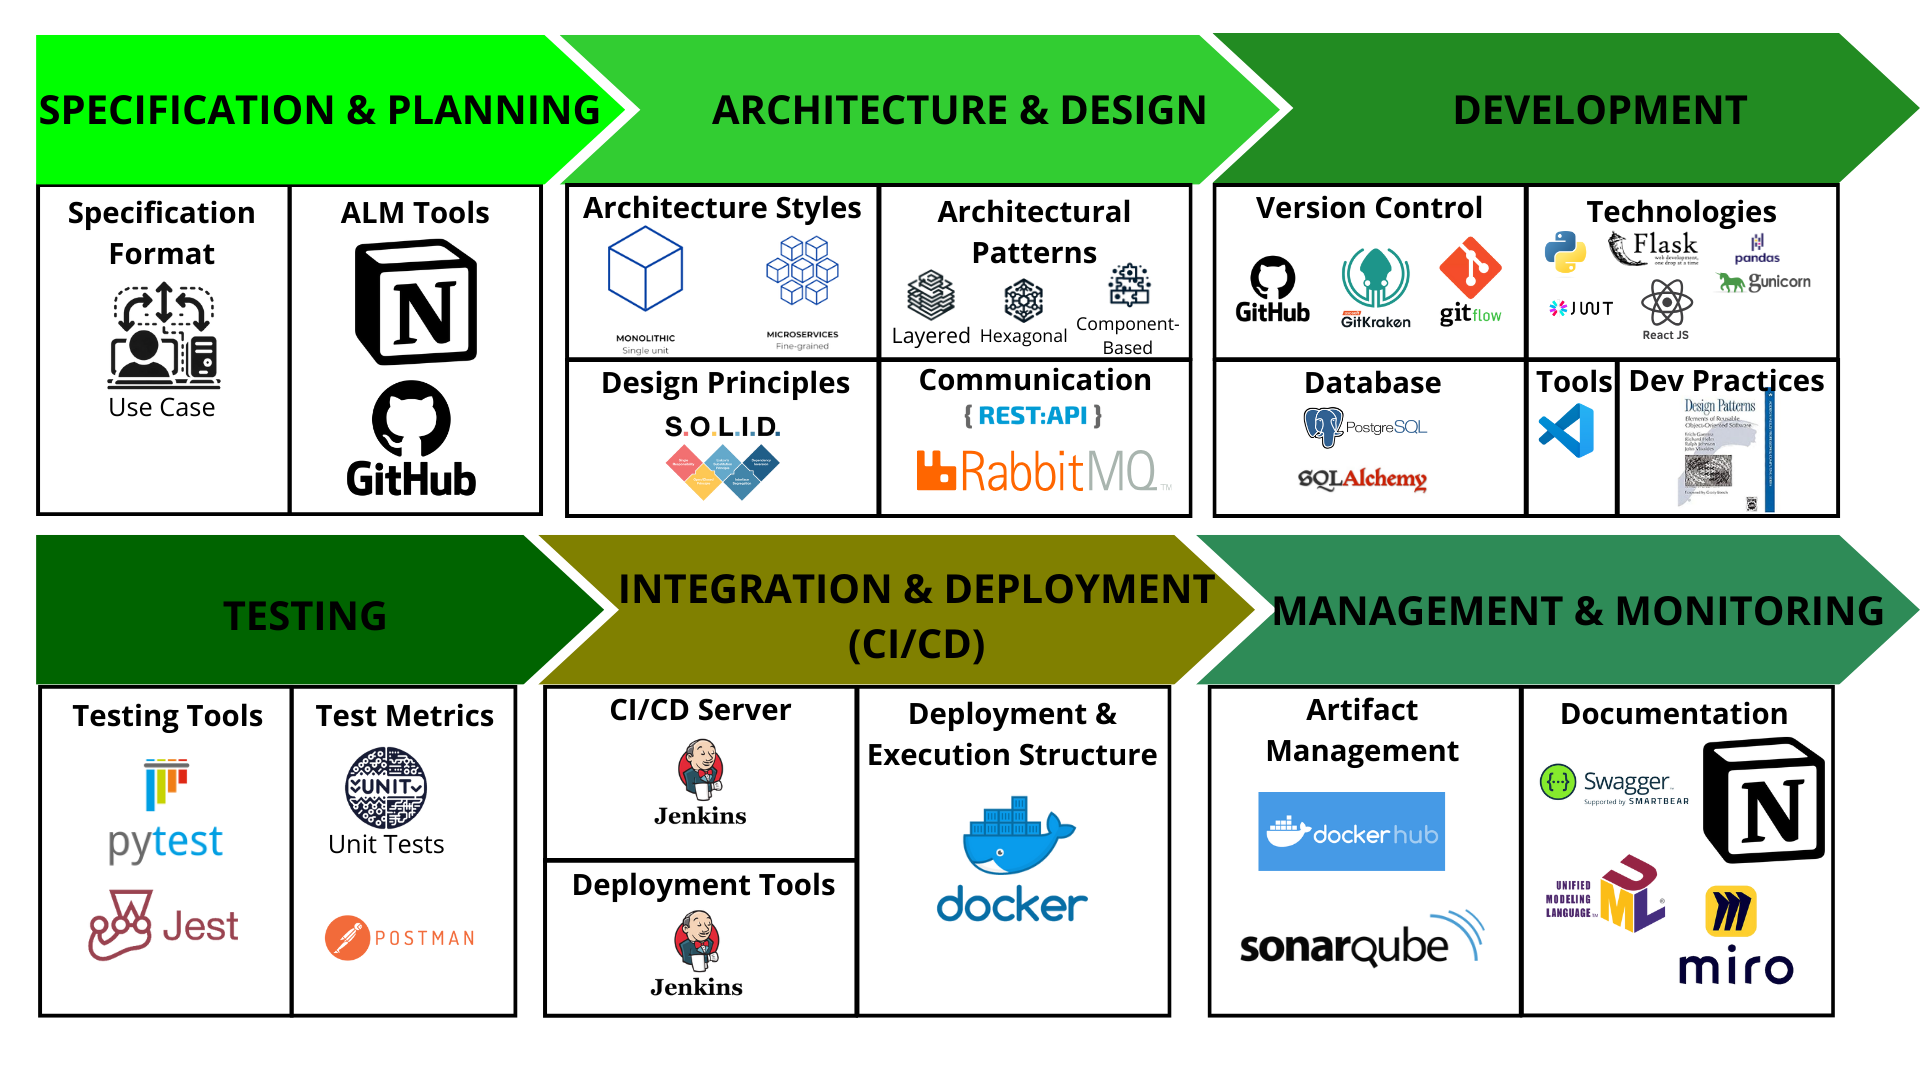
\includegraphics[width=1\linewidth]{Textuais/FinTrackr.png}
	\caption{tecnologias, técnicas, design, estilo arquiteturas}
	\label{fig:fintrackr_technologies}
\end{figure}

\section{Requisitos}

\subsection{Requisitos Funcionais}
\begin{enumerate}
	\item \textbf{RF01}: Implementação de um sistema de autenticação robusto e seguro, permitindo registro, login, recuperação de senha e gerenciamento de perfil.
	\item \textbf{RF02}: Facilitar o gerenciamento de informações do perfil do usuário, incluindo visualização, adição, atualização e exclusão de dados como nome, endereço e telefone.
	\item \textbf{RF03}: Permitir o registro de transações financeiras, categorizando-as como receitas ou despesas e associando detalhes pertinentes.
	\item \textbf{RF04}: Habilitar a criação, edição e exclusão de categorias de transações, associando detalhes como nome, cor e ícone.
	\item \textbf{RF05}: Proporcionar a definição e monitoramento de orçamentos mensais por categoria, mostrando gastos realizados e disponíveis.
	\item \textbf{RF06}: Prover um dashboard que apresente um resumo financeiro, incluindo saldo em contas, resumo de orçamentos, gastos por categoria e balanço geral.
	\item \textbf{RF07}: Integrar com um microserviço para permitir a importação de faturas bancárias em formato .csv, iniciando pelo Bradesco.
	\item \textbf{RF08}: Facilitar o gerenciamento de cartões de crédito, incluindo registro de faturas e lançamentos associados.
	\item \textbf{RF09}: Oferecer uma visualização detalhada do histórico de saldo, mostrando a evolução financeira do usuário.
	\item \textbf{RF10}: Permitir o registro e gerenciamento de bancos associados às contas do usuário.
\end{enumerate}

\subsection{Requisitos Não Funcionais}
\begin{enumerate}
	\item \textbf{RNF01}: A interface do sistema deve ser intuitiva e organizada.
	\item \textbf{RNF02}: Adaptabilidade para diferentes dispositivos, mantendo funcionalidade e design em smartphones, tablets e desktops.
	\item \textbf{RNF03}: Fornecer feedback claro e direto ao usuário em todas as interações.
	\item \textbf{RNF04}: Código-fonte bem estruturado, seguindo padrões reconhecidos de programação.
	\item \textbf{RNF05}: As operações do sistema devem ser otimizadas para resposta rápida, garantindo eficiência.
\end{enumerate}

\section{Regras de Negócio}
\begin{enumerate}
	\item \textbf{RN01}: Transações devem ser associadas a uma categoria.
	\item \textbf{RN02}: Cartões e contas com faturas ou transações associadas não podem ser excluídos.
	\item \textbf{RN03}: Categorias com transações associadas não podem ser excluídas.
	\item \textbf{RN04}: Ao dividir despesas em múltiplas categorias, o valor associado a cada categoria deve ser especificado.
	\item \textbf{RN05}: O total de valores associados em uma transação dividida entre categorias deve igualar o valor total da transação.
	\item \textbf{RN06}: Orçamentos não podem ter valores negativos.
	\item \textbf{RN07}: Despesas em cartões de crédito devem ser associadas à fatura corrente.
	\item \textbf{RN08}: Transações em contas impactam o saldo da mesma.
	\item \textbf{RN09}: Transações não podem ter datas futuras.
	\item \textbf{RN10}: Importações de faturas via .csv devem permitir edição pós-importação.
	\item \textbf{RN11}: Faturas de cartões possuem status baseados em datas de vencimento e pagamentos.
	\item \textbf{RN12}: Usuários devem ser notificados ao atingir ou exceder orçamentos.
	\item \textbf{RN13}: Categorias não podem ser duplicadas em uma transação dividida.
	\item \textbf{RN14}: Saldos negativos em contas devem ser prevenidos, a menos que permitidos.
	\item \textbf{RN15}: Informações de cartões ou contas duplicadas não são permitidas.
	\item \textbf{RN16}: Os usuários devem fornecer um email e senha válidos para se autenticar no sistema.
	\item \textbf{RN17}: Senhas devem ter um mínimo de 8 caracteres e conter pelo menos uma letra maiúscula, uma letra minúscula, um número e um caractere especial.
	\item \textbf{RN18}: Para recuperação de senha, o usuário deve confirmar sua identidade através de um link enviado ao seu email registrado.
	\item \textbf{RN19}: O email fornecido pelo usuário durante o registro ou atualização do perfil deve ser único no sistema.
	\item \textbf{RN20}: Para alterar a senha, o usuário deve fornecer a senha atual para confirmação.
\end{enumerate}

\section{Casos de Uso}

\subsection*{UC01: Autenticação no Sistema}
Apêndice \ref{apendiceUC01}

\subsection*{UC02: Gerenciar Perfil}
Apêndice \ref{apendiceUC02}

\subsection*{UC03: Registrar e Categorizar Transações}
Apêndice \ref{apendiceUC03}

\subsection*{UC04: Gerenciar Categorias}
Apêndice \ref{apendiceUC04}

\subsection*{UC05: Gerenciar Orçamentos}
Apêndice \ref{apendiceUC05}

\subsection*{UC06: Visualizar Dashboard Financeiro}
Apêndice \ref{apendiceUC06}

\subsection*{UC07: Importar Faturas}
Apêndice \ref{apendiceUC07}

\subsection*{UC08: Gerenciar Cartões e Faturas}
Apêndice \ref{apendiceUC08}

\subsection*{UC09: Acompanhar Evolução de Saldo}
Apêndice \ref{apendiceUC09}

\subsection*{UC10: Gerenciar Bancos}
Apêndice \ref{apendiceUC10}


\subsection*{UC11: Definir Mês de Referência para Transações}
Apêndice \ref{apendiceUC11}

\end{itemize}